\documentclass[handout,nooutcomes]{ximera}
%% handout
%% space
%% newpage
%% numbers
%% nooutcomes

%I added the commands here so that I would't have to keep looking them up
%\newcommand{\RR}{\mathbb R}
%\renewcommand{\d}{\,d}
%\newcommand{\dd}[2][]{\frac{d #1}{d #2}}
%\renewcommand{\l}{\ell}
%\newcommand{\ddx}{\frac{d}{dx}}
%\everymath{\displaystyle}
%\newcommand{\dfn}{\textbf}
%\newcommand{\eval}[1]{\bigg[ #1 \bigg]}

%\begin{image}
%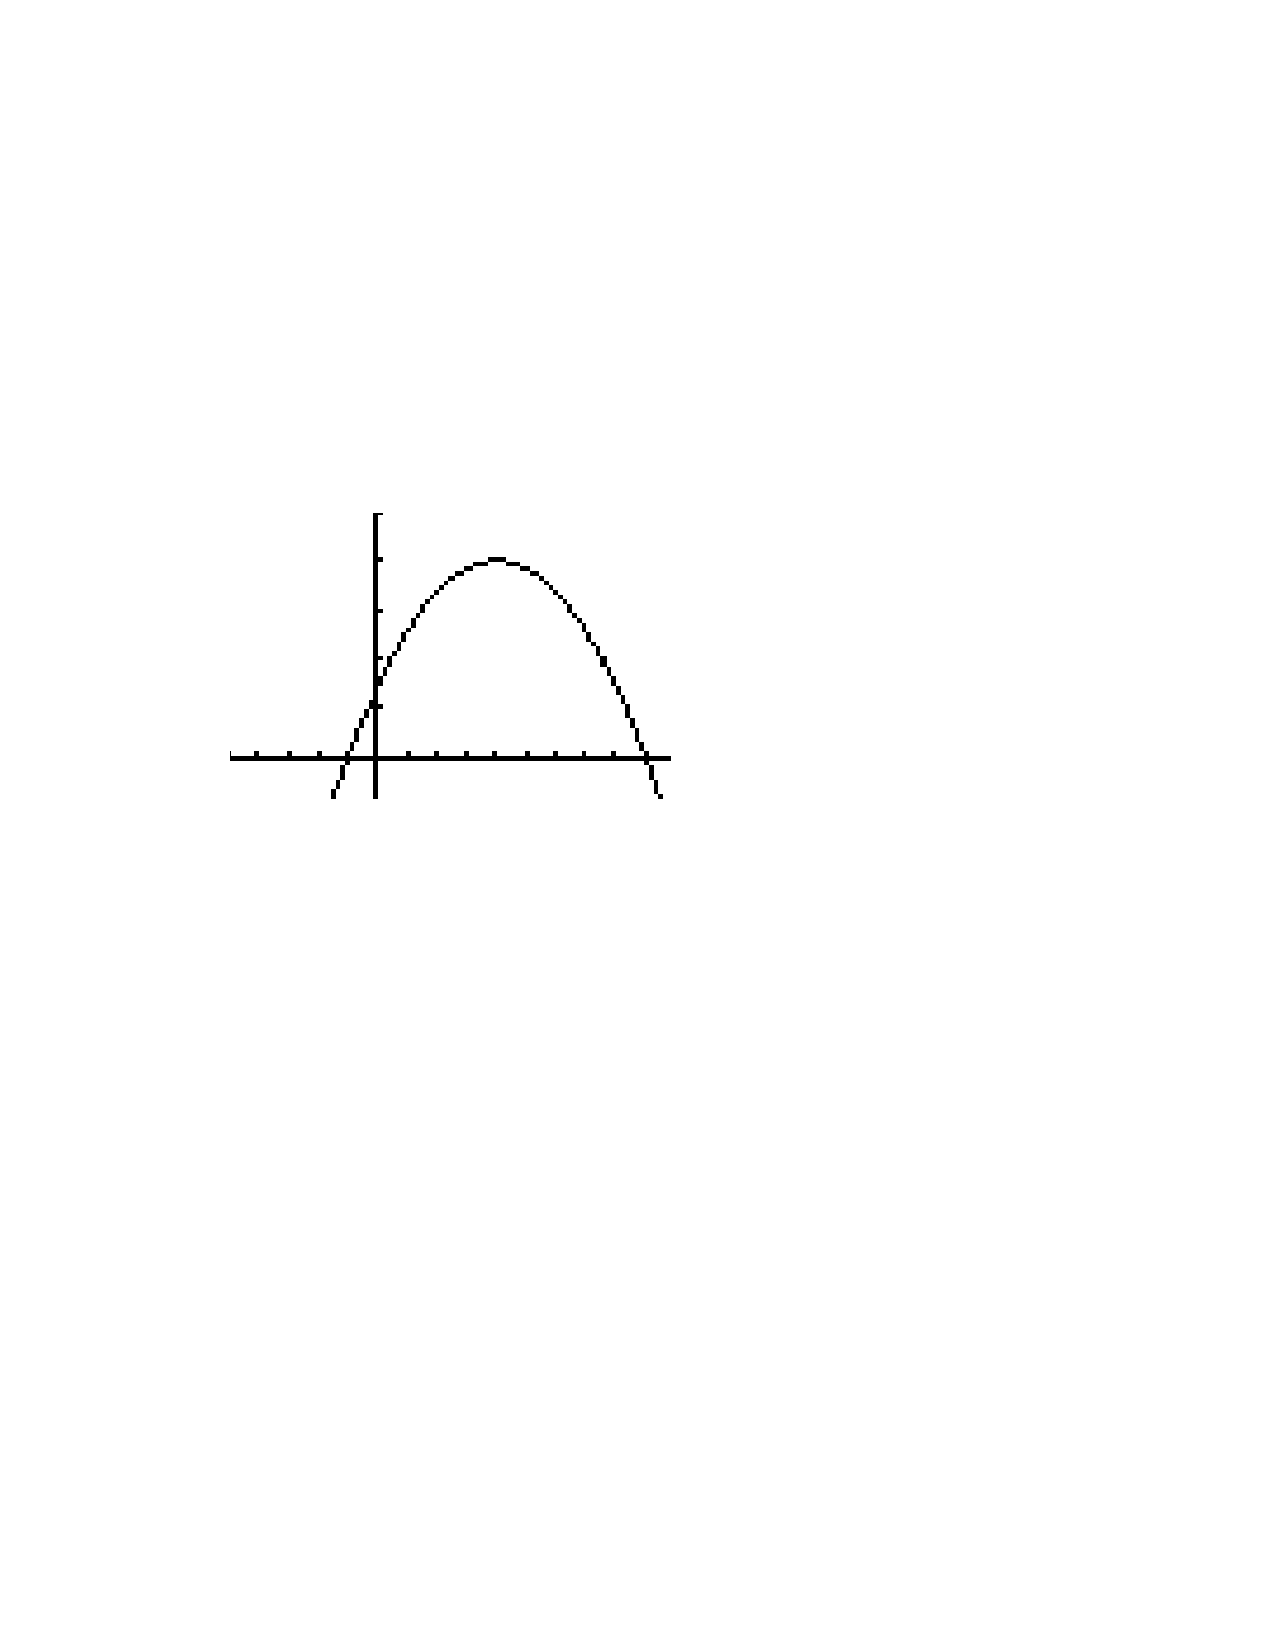
\includegraphics[trim= 170 420 250 180]{Figure1.pdf}
%\end{image}


\newcommand{\RR}{\mathbb R}
\renewcommand{\d}{\,d}
\newcommand{\dd}[2][]{\frac{d #1}{d #2}}
\renewcommand{\l}{\ell}
\newcommand{\ddx}{\frac{d}{dx}}
\newcommand{\dfn}{\textbf}
\newcommand{\eval}[1]{\bigg[ #1 \bigg]}

\usepackage{multicol}

\renewenvironment{freeResponse}{
\ifhandout\setbox0\vbox\bgroup\else
\begin{trivlist}\item[\hskip \labelsep\bfseries Solution:\hspace{2ex}]
\fi}
{\ifhandout\egroup\else
\end{trivlist}
\fi} %% we can turn off input when making a master document

\title{Recitation \#18 - 4.4 Optimization Problems}  

\begin{document}
\begin{abstract}		\end{abstract}
\maketitle

\section*{Warm up:} 
Suppose you want to maximize a continuous function on a closed interval, but you find that it only has one local extremum on the interval which happens to be a local minimum.  Where else should you check for the solution?  
		\begin{freeResponse}
		The endpoints.
		\end{freeResponse}	
		
		
		

	
	
	
	
	

\section*{Group work:}



%problem 1
\begin{problem}
A rectangular flower garden with an area of $30 \, m^2$ is surrounded by a grass border $1 \, m$ wide on two sides and $2 \, m$ wide on the other two sides (see figure).  What dimensions of the garden minimize the combined area of the garden and borders?

	\begin{image}
	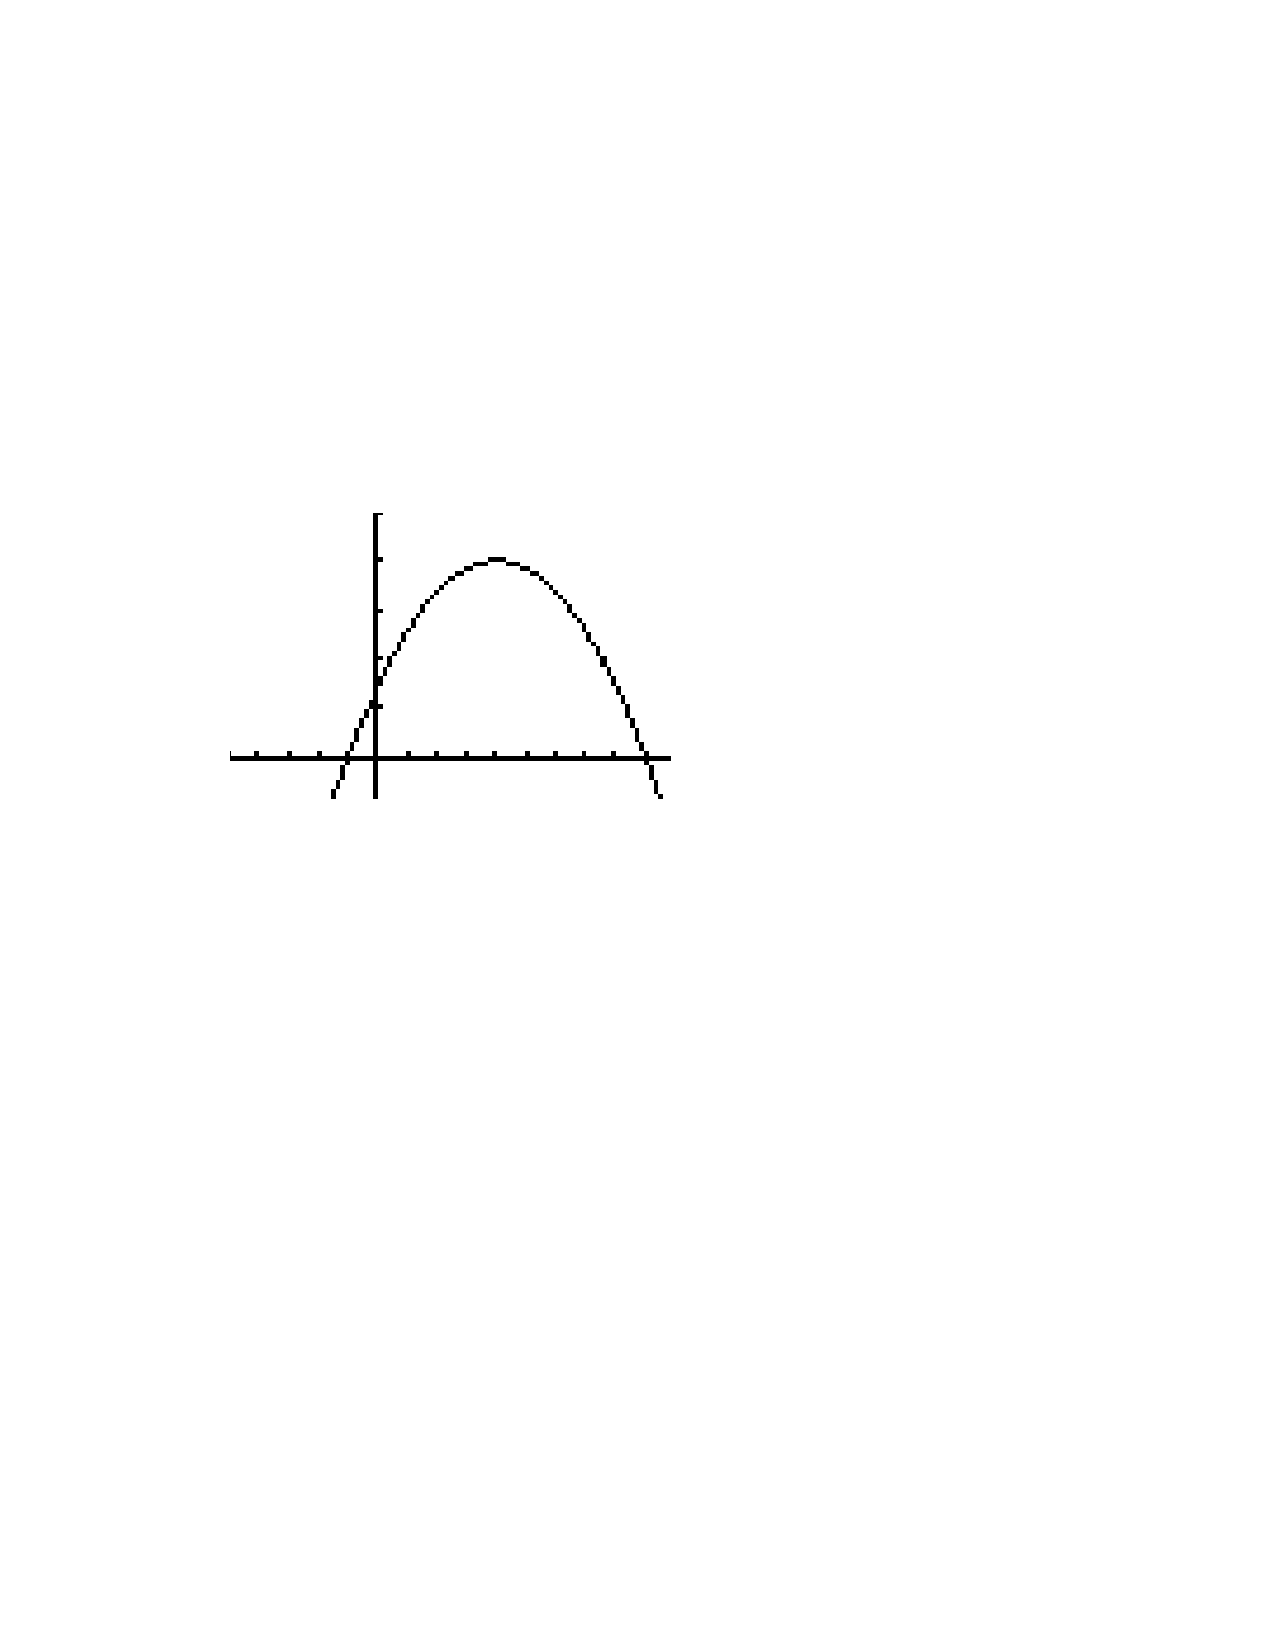
\includegraphics[trim= 100 480 250 250]{Figure1.pdf}
	\end{image}

	\begin{enumerate}
	
	%part a
	\item  Label the picture with variables.
		\begin{freeResponse}
		\begin{image}
		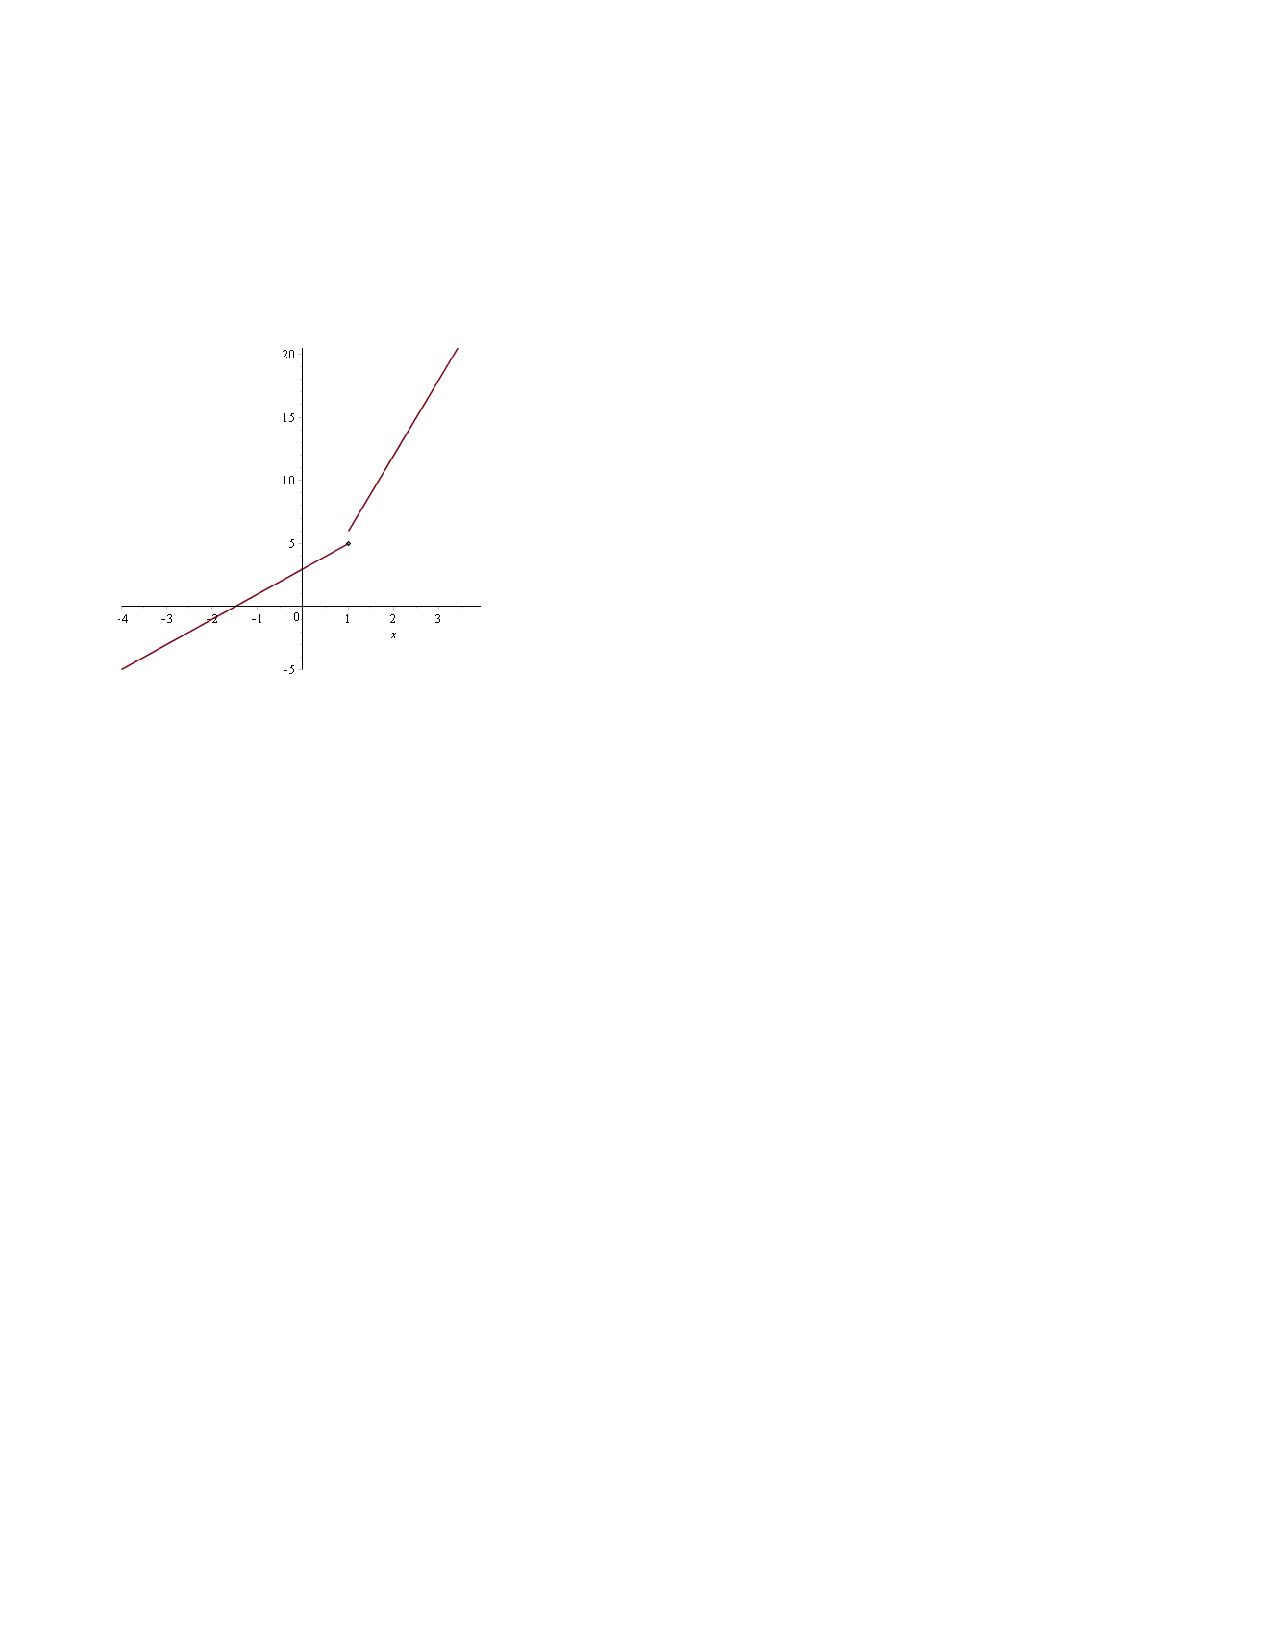
\includegraphics[trim= 640 500 250 210]{Figure6.pdf}
		\end{image}
		\end{freeResponse}
		
		
		
	%part b
	\item  What are you trying to maximize or minimize?  Write an equation for it in terms of the variables from (a).
		\begin{freeResponse}
		We want to minimize the combined area of the garden and border.  If $A$ denotes this area, then an equation for $A$ is
		$$ A = (x+4)(y+2) $$
		\end{freeResponse}
		
		
		
	%part c
	\item  What is your constraint?  Write a constraint equation in terms of the variables from (a).
		\begin{freeResponse}
		We know that the area of the flower garden is $30 \, m^2$.  So our constraint equation is
		$$ xy = 30 $$
		\end{freeResponse}
		
		
		
	%part d
	\item  Reduce your optimization equation to one variable using the constraint equation.
		\begin{freeResponse}
		$$ x = \frac{30}{y} \quad (\text{Note that } y \neq 0) $$
		\begin{align}
		A &= \left( \frac{30}{y} + 4 \right)(y+2) \\
		&= 30 + 4y + \frac{60}{y} + 8 \\
		&=4y + \frac{60}{y} + 38 \label{eqn3}
		\end{align}
		\end{freeResponse}
		
		
		
	%part e
	\item  What is the interval on which your variable makes sense?  Is it open or closed?  What does this mean for the method of finding the absolute max or min?
		\begin{freeResponse}
		$0 < y < \infty$, which is an open interval.  So we need there to only be one critical point to equation \eqref{eqn3} in the domain of $y$, and then we need to show that this critical point is a local minimum.  This will imply that the critical point is an absolute minimum (since there is only one critical point).  
		\end{freeResponse}
		
		
		
	%part f
	\item  Use the appropriate method to find and justify your absolute extremum.
		\begin{freeResponse}
		We need to differentiate equation \eqref{eqn3} with respect to $y$, set this derivative equal to $0$, and then solve:
		$$ \dd[A]{y} = 4 - \frac{60}{y^2} :=0 $$
		$$ \frac{60}{y^2} = 4 $$
		$$ 4y^2 = 60 $$
		$$ y^2 = 15 $$
		$$ y = \pm \sqrt{15} $$
		Since $-\sqrt{15}$ is not in our domain, the only critical point of $A(y)$ in the interval $(0,\infty)$ is $\sqrt{15}$.  
		Thus, if $y=\sqrt{15}$ is a local minimum for $A$, then it will be an absolute minimum.  
		Using the $2^{nd}$ derivative test:
		$$ \dd[^2A]{y^2} = \frac{120}{y^3} $$
		$$ \eval{\dd[^2A]{y^2}}_{y=\sqrt{15}} = \frac{120}{15 \sqrt{15}} > 0. $$
		
		Since $A(y)$ is concave up at $y=\sqrt{15}$, this point is a local (and thus, absolute) minimum of $A(y)$.  
		Note that we also could have used the first derivative test to show that $y=\sqrt{15}$ was a local minimum of $A$.
		
		\end{freeResponse}
		
		
		
	%part g
	\item  Be sure to answer the question asked in the original problem.
		\begin{freeResponse}
		Since $y=\sqrt{15} \, m$, we have that
		$$ x = \frac{30}{y} = \frac{30}{\sqrt{15}} = \frac{30 \sqrt{15}}{15} = 2 \sqrt{15} \, m $$
		\end{freeResponse}
		
		
		
	\end{enumerate}
		
		
\end{problem}
















%problem 2
\begin{problem}
A cone is constructed by cutting a sector from a circular sheet of metal with radius 20.  The cut sheet is then folded and welded.  Find the radius and height of the cone with maximum volume that can be formed this way.

	\begin{image}
	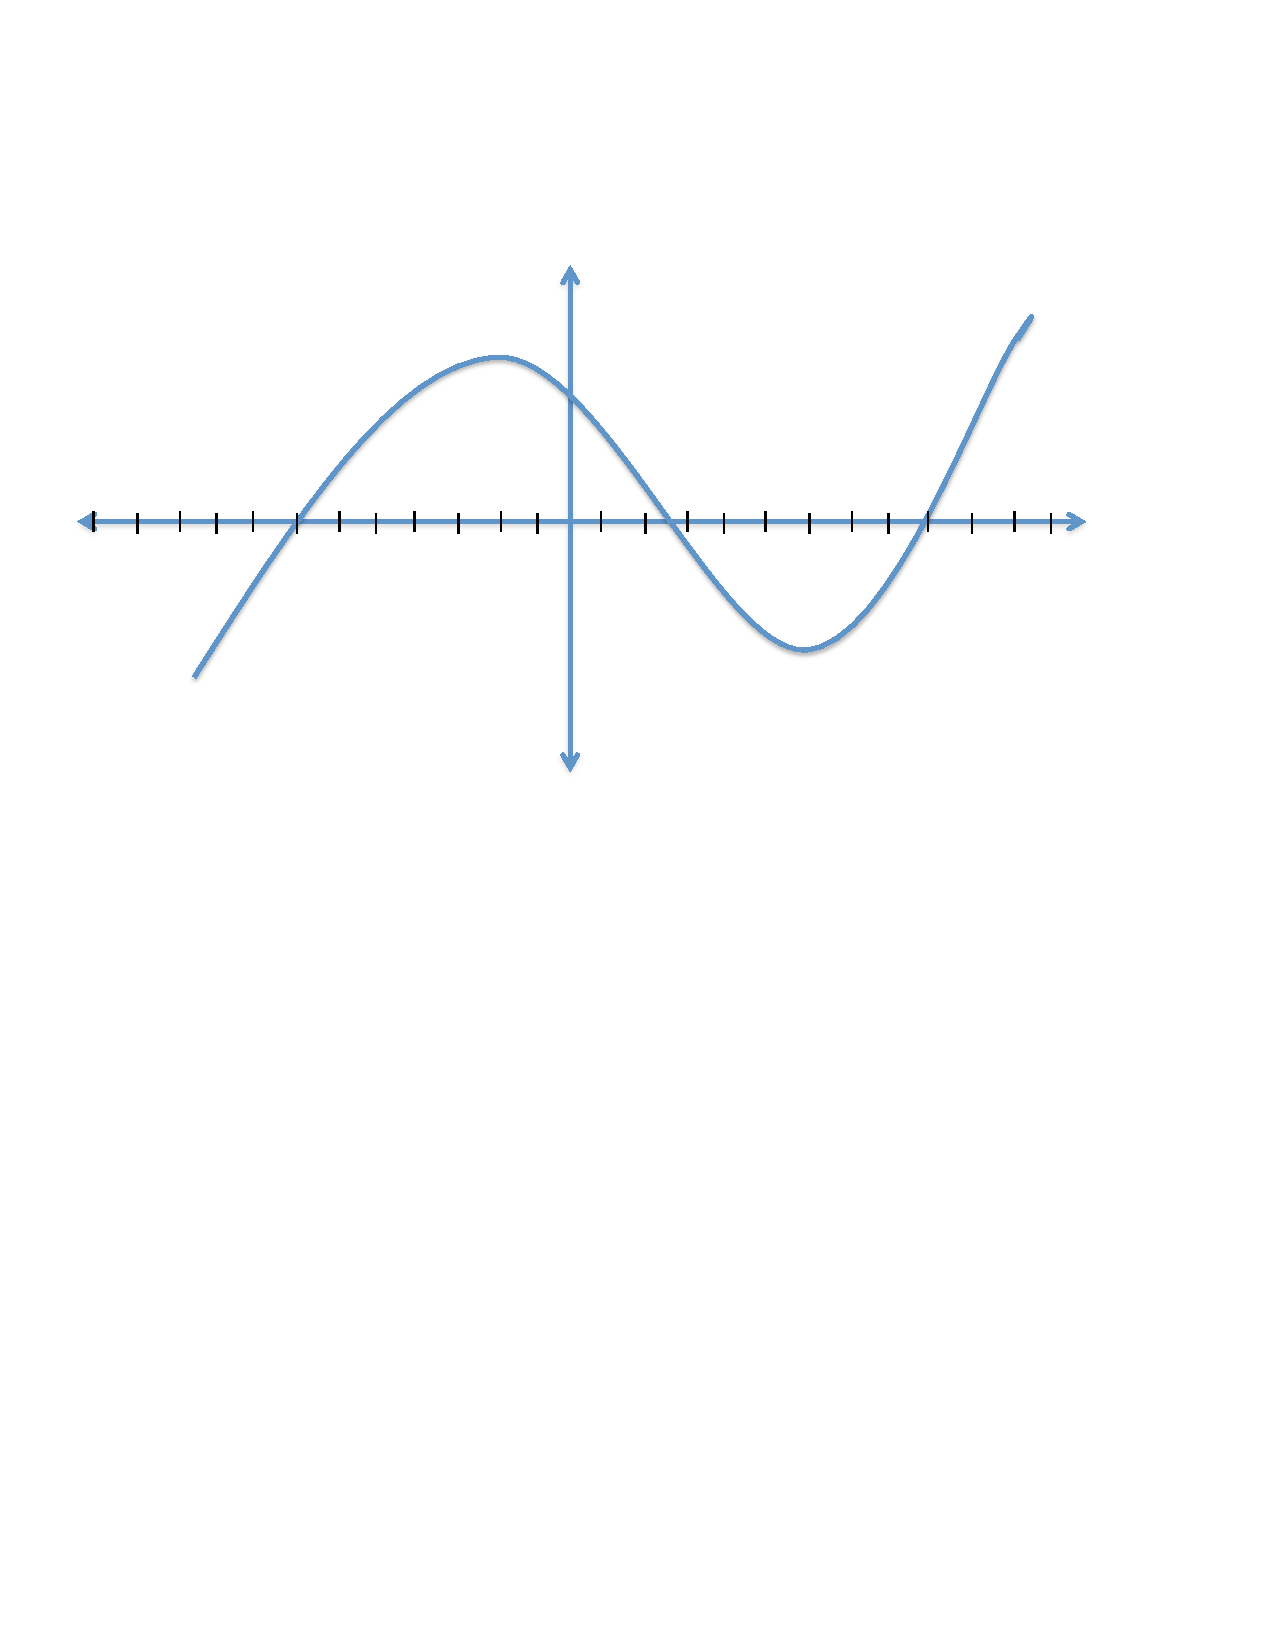
\includegraphics[trim= 100 530 250 190]{Figure2.pdf}
	\end{image}
	
		\begin{freeResponse}
		First, recall that the volume of a cone is
		\begin{equation}\label{cone volume}
		V = \frac{1}{3} \pi r^2 h
		\end{equation}
		
		Equation \eqref{cone volume} has two variables, $r$ and $h$.  
		So we need to find a constraint equation.  
		Notice that the length of the cone is a fixed length of 20.  
		So using Pythagorean's Theorem we have that:
		\begin{equation}\label{constraint}
		r^2 + h^2 = 20^2 = 400
		\end{equation}
		
		Solving equation \eqref{constraint} for $r^2$, we get $r^2 = 400 - h^2$.  
		Plugging this into equation \eqref{cone volume} gives
		\begin{equation}\label{V(h)}
		V = \frac{1}{3} \pi (400-h^2) h = \frac{1}{3} \pi (400h - h^3) 
		\end{equation}
		Note that, due to the settings of the problem, the domain for $h$ is $[0,20]$.  
		
		It is worth pointing out that it is a lot easier algebraically to solve for $r^2$ in equation \eqref{constraint} 
		and then plug into equation \eqref{cone volume} instead of doing the same thing for $h$.
		
		Now we need to differentiate equation \eqref{V(h)} with respect to $h$, set this equal to $0$, and solve for $h$.
		$$ \dd[V]{h} = \frac{1}{3} \pi (400 - 3h^2) := 0 $$
		$$ 400 - 3h^2 = 0 $$
		$$ 3h^2 = 400 $$
		$$ h^2 = \frac{400}{3} $$
		$$ h = \pm \sqrt{\frac{400}{3}} = \pm \frac{20}{\sqrt{3}} $$
		but $- \frac{20}{\sqrt{3}}$ is not in our domain for $h$, and so the only critical point for $V(h)$ is $h = \frac{20}{\sqrt{3}}$.  
		We need to show that this is an absolute maximum for $V(h)$ on $[0,20]$.  
		Since $[0,20]$ is a closed interval, we can just evaluate $V(h)$ at $h=0, \frac{20}{\sqrt{3}}, 20$.  
		\begin{align}
		V(0) &= \frac{1}{3} \pi (0-0) = 0 \\
		V \left( \frac{20}{\sqrt{3}} \right) &= \frac{1}{3} \pi \left( \frac{20^3}{\sqrt{3}} - \frac{20^3}{\left( \sqrt{3} \right)^3} \right) > 0 \label{inequality} \\
		V(20) &= \frac{1}{3} \pi (20^3 - 20^3) = 0 
		\end{align}
		
		Thus $h=\frac{20}{\sqrt{3}}$ maximizes the volume of the cone.  Then 
		$$r^2 = 400 - h^2 = 400 - \left( \frac{20}{\sqrt{3}} \right)^2 = 400 - \frac{400}{3} = \frac{800}{3}$$
		and so
		$$ r = 20 \sqrt{\frac{2}{3}}. $$
		
		If you are not comfortable with inequality \eqref{inequality} above without a calculator, then a nice alternative is to use the second derivative test instead to check that $h=\frac{20}{\sqrt{3}}$ maximizes the volume of the cone.  This works since this is the only critical point in the domain of $h$.  To do this, compute
		$$ \dd[^2V]{h^2} = \frac{1}{3} \pi (-6h) $$
		$$ \eval{\dd[^2V]{h^2}}_{h=\frac{20}{\sqrt{3}}} = \frac{1}{3} \pi \left( -6 \left(\frac{20}{\sqrt{3}} \right) \right) < 0 $$
		and thus this value for $h$ gives a local (and therefore, absolute) maximum value for $V(h)$.  
		
		\end{freeResponse}
		
		
		

\end{problem}
	


	
	
\begin{center}	\dfn{Extra Problems (No solutions will be provided for these problems)}	\end{center}
	
			
			

%problem 3
\begin{problem}
What is the length of the longest pole that can be carried horizontally around a corner at which a $3-ft$ corridor and a $4-ft$ corridor meet at right angles? (challenging)
\end{problem}



%problem 4
\begin{problem}
A covered metal triangular trough is constructed as follows:  A square-shaped sheet of metal which is $70 \, cm$ wide and long square is folded along the center.  Next, two pieces of metal in the shape of isosceles triangles are welded to the ends.  Finally, a metal cover is attached to the top.  Find the largest and smallest possible surface area that such a constructed trough can have (Hint:  Find the surface area as a function of half the angle formed by the bottom corner of the isosceles triangles)

		\begin{image}
		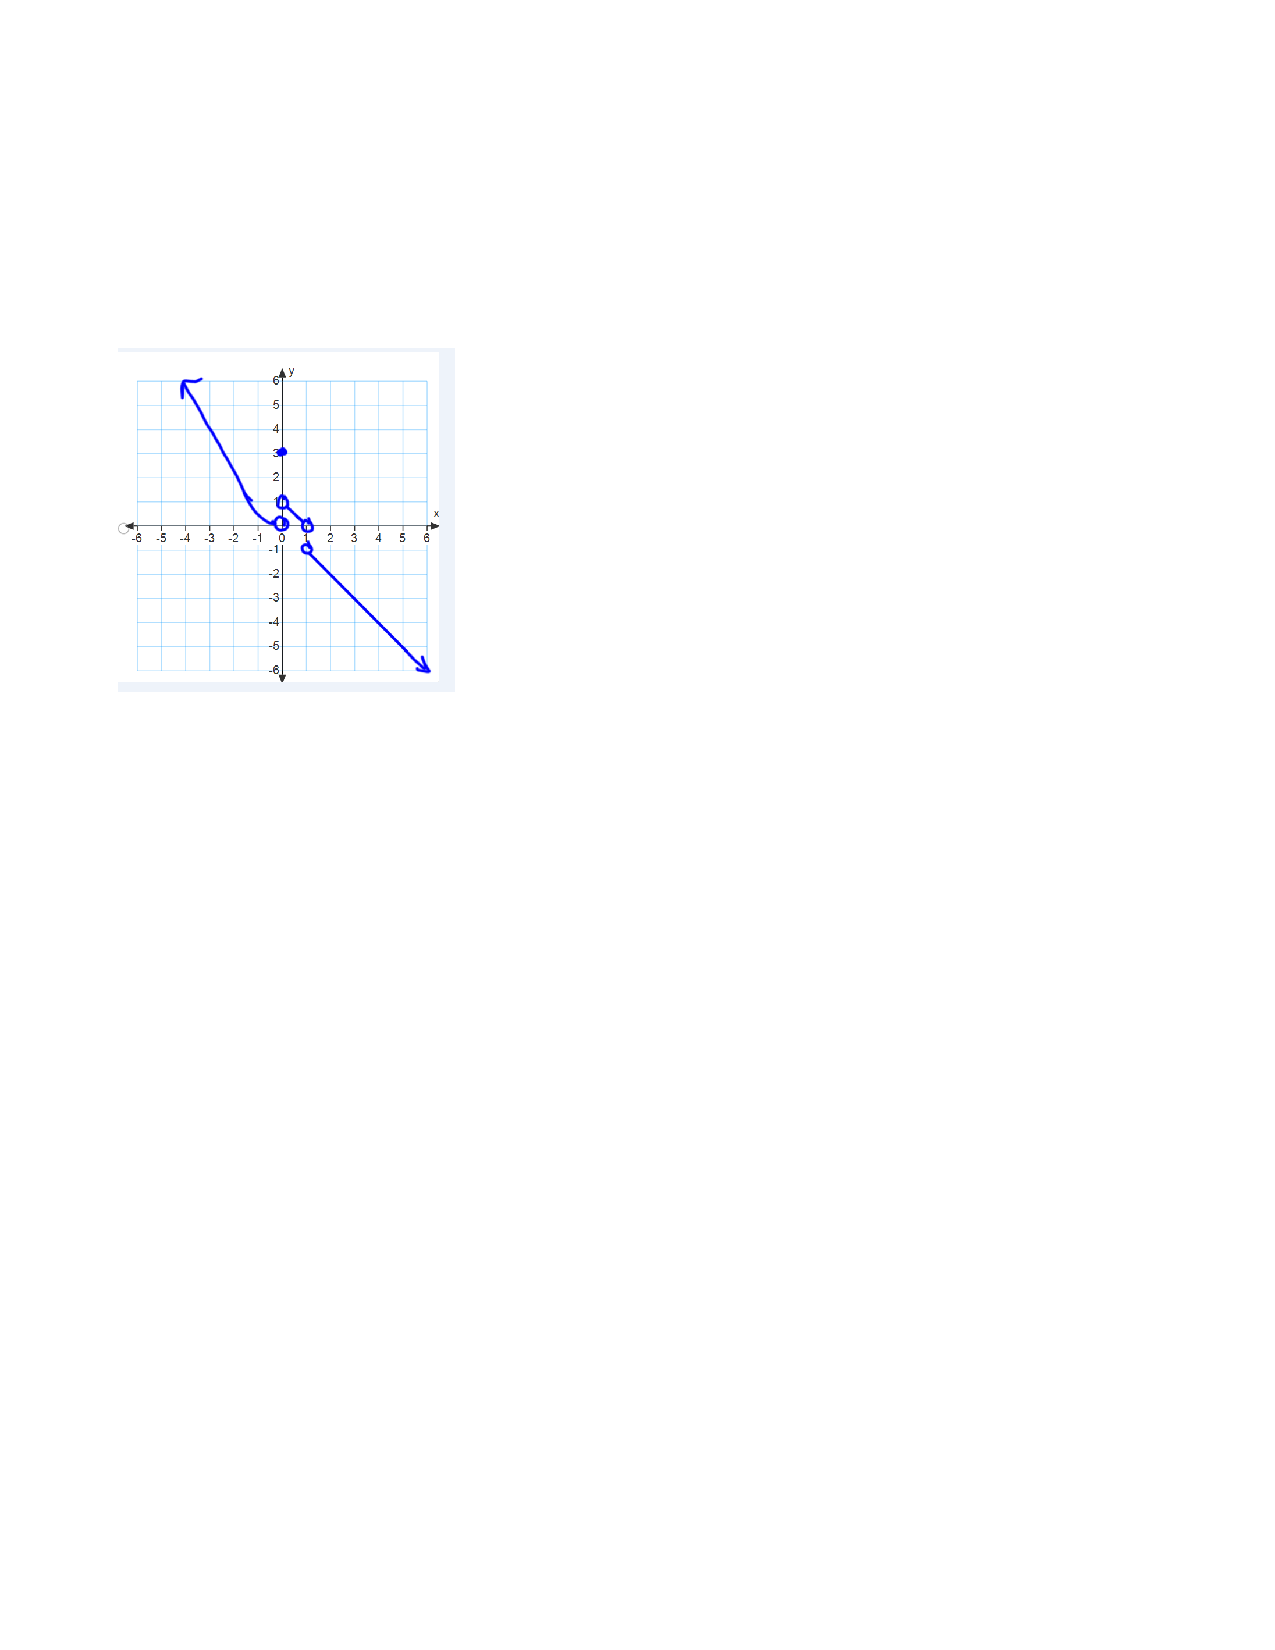
\includegraphics[trim= 100 550 250 190]{Figure3.pdf}
		\end{image}
\end{problem}



%problem 5
\begin{problem}
Find the largest total surface area (including top and bottom) of a cylinder inscribed in a cone of radius $6$ and height $16$. 

		\begin{image}
		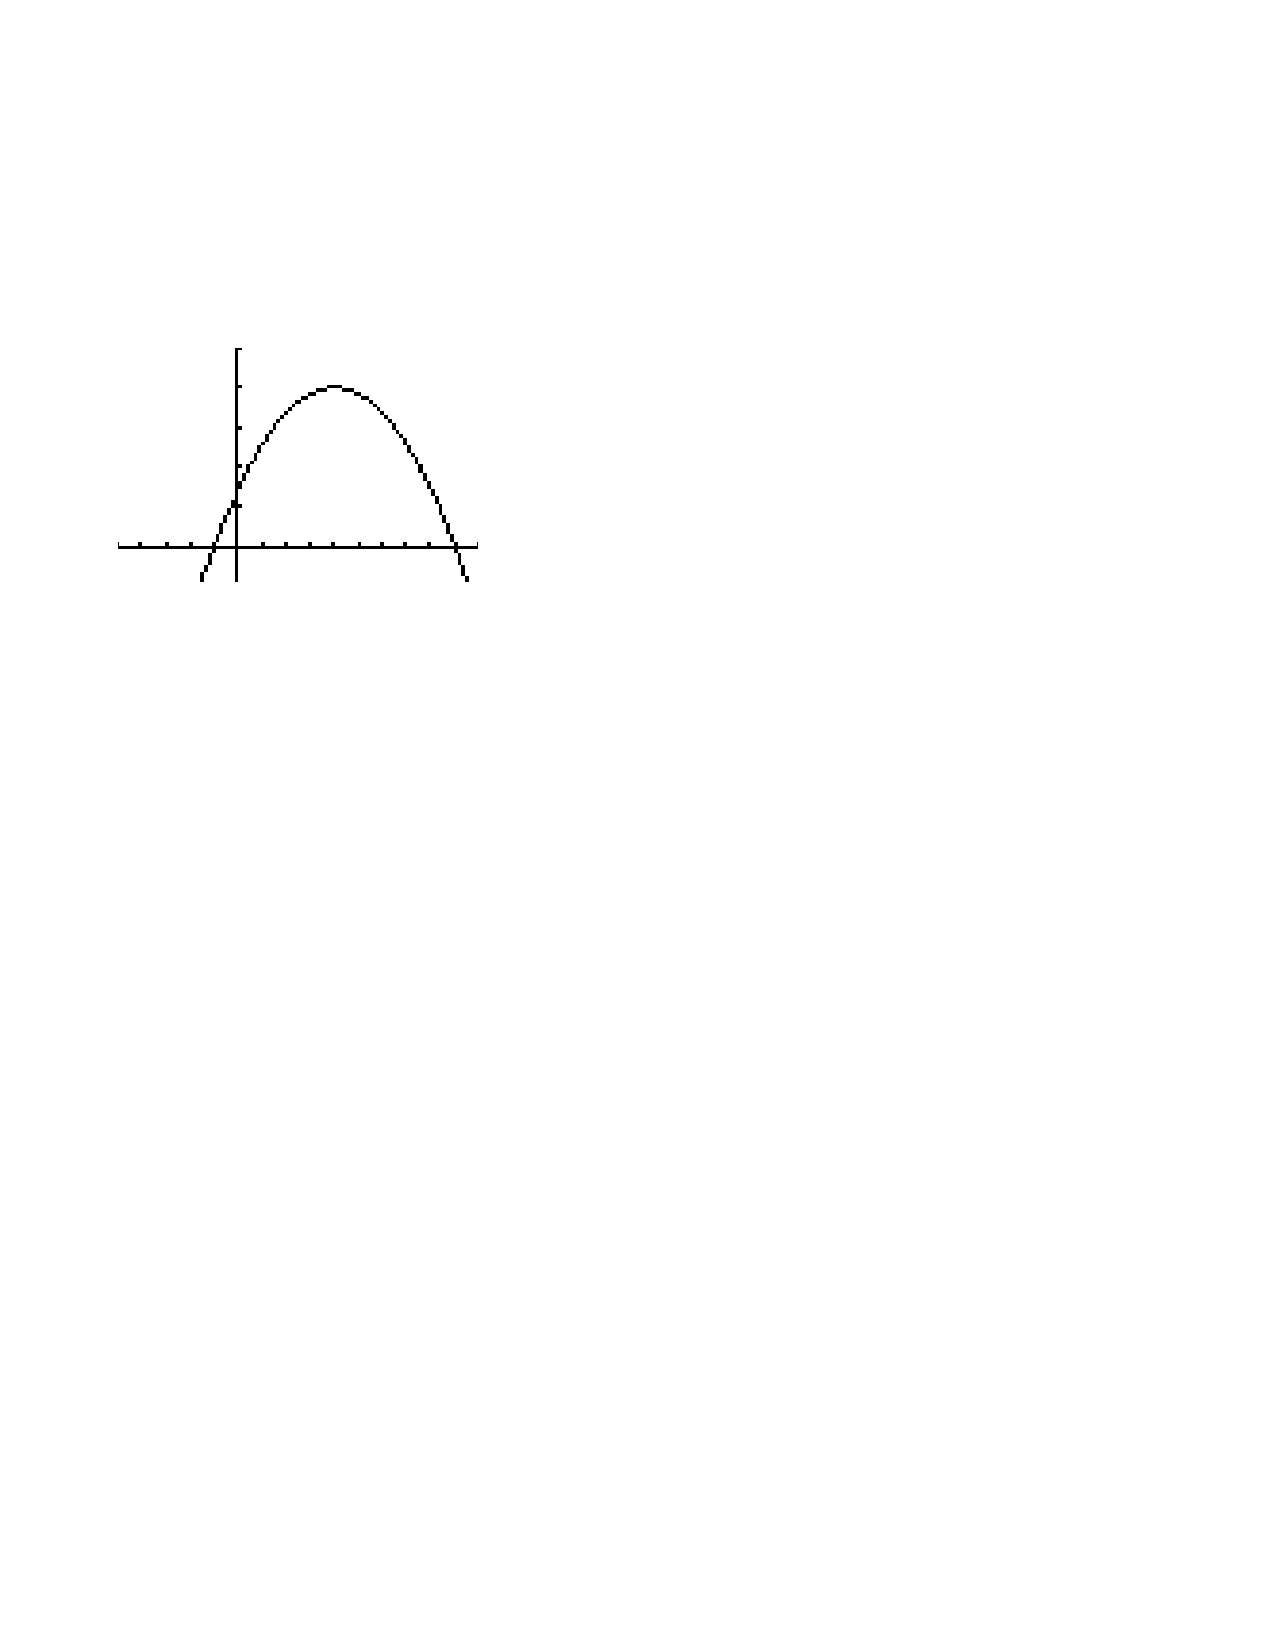
\includegraphics[trim= 100 540 250 190]{Figure4.pdf}
		\end{image}
\end{problem}



%problem 6
\begin{problem}
A man with a boat is located at point $P$ on the shore of a circular lake of radius $6$ miles.  He wants to reach point $Q$ on the shore diametrically opposite to $P$ as quickly as possible.  He plans to paddle his boat at an angle $\theta$ to some point $R$ on the shore, then walk along the shore to $Q$.  If he can paddle $3.2$ mph and walk at $3.7$ mph, what is the shortest possible time it will take him to reach $Q$? (challenging, but like an example in the book)

		\begin{image}
		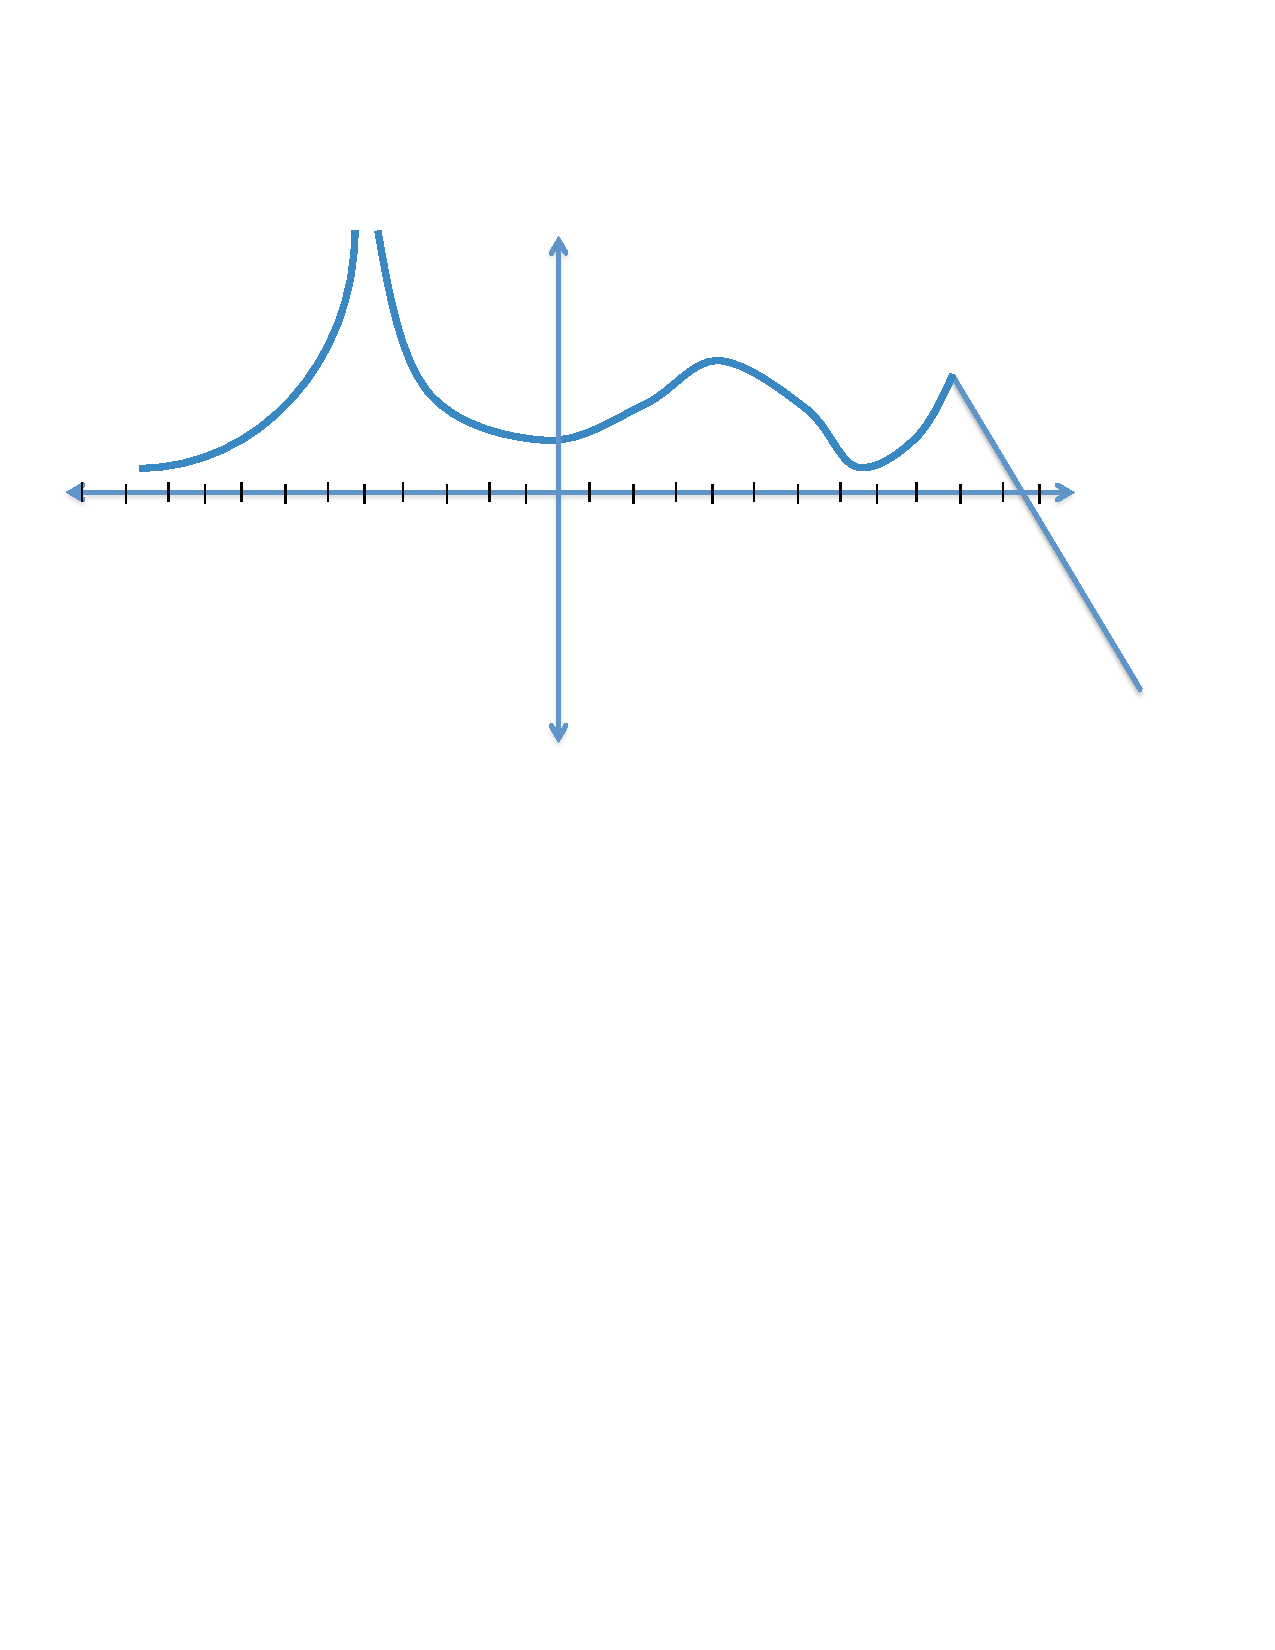
\includegraphics[trim= 100 540 250 190]{Figure5.pdf}
		\end{image}
\end{problem}



%problem 7
\begin{problem}
What point on the parabola $y=5-x^2$ is closest to the point $(4,7)$?  
\end{problem}



%problem 8
\begin{problem}
Waste-free box: Make an open-topped box by cutting congruent squares from the corners of an $8.5$ by $11$ inch sheet of paper.  Then tape together the four cut-out squares to make a box with no top or bottom (e.g., a pencil holder).  What is the maximum combined volume of the two figures?  Do also for a $6$ by $10$ inch piece of paper.
\end{problem}



%problem 9
\begin{problem}
Rectangles beneath a line

	\begin{enumerate}
	
	\item  A rectangle is constructed with one side on the positive $x$-axis, one side on the positive $y$-axis, and the vertex opposite the origin on the line $y=10-2x$.  What dimensions maximize the area of the rectangle?  What is the maximum area?
	
	\item  Is it possible to construct a rectangle with a greater area than that found in part (a) by placing one side of the rectangle on the line $y=10-2x$, and the other two vertices not on that line on the positive $x$ and $y$-axes?  Find the dimensions of the rectangle of maximum area that can be constructed in this way. (challenging)
	
	\end{enumerate}
\end{problem}



%problem 10
\begin{problem}
A right cylinder is placed inside a cone of radius $R$ and height $H$ so that the base of the cylinder lies on the base of the cone.

	\begin{enumerate}
	
	\item  Find the dimensions of the cylinder with maximum volume.  Specifically, show that the volume of this cylinder is $\frac{4}{9}$ times the volume of the cone.
	
	\item  Find the dimensions of the cylinder with maximum lateral surface area (area of the curved surface).
	
	\end{enumerate}
\end{problem}



%problem 11
\begin{problem}
Suppose you are standing in a field near a straight section of railroad tracks just as the locomotive of a train passes the point nearest to you, which is $\frac{1}{4}$ of a mile away.  The train, with length $\frac{1}{3}$ mi, is traveling at $20$ mi/hr.  If you start running in a straight line across the field, how slowly can you run and still catch the train?  In which direction should you run? (challenging)
\end{problem}






	
	
	
	
	
	
	
	
	

	










								
				
				
	














\end{document} 


















